%%
%% Automatically generated file from DocOnce source
%% (https://github.com/hplgit/doconce/)
%%

% #define PREAMBLE

% #ifdef PREAMBLE
%-------------------- begin preamble ----------------------

\documentclass[%
oneside,                 % oneside: electronic viewing, twoside: printing
final,                   % draft: marks overfull hboxes, figures with paths
10pt]{article}

\listfiles               %  print all files needed to compile this document

\usepackage{relsize,makeidx,color,setspace,amsmath,amsfonts,amssymb}
\usepackage[table]{xcolor}
\usepackage{bm,ltablex,microtype}

\usepackage[pdftex]{graphicx}
\usepackage{fancyvrb}

\usepackage[T1]{fontenc}
%\usepackage[latin1]{inputenc}
\usepackage{ucs}
\usepackage[utf8x]{inputenc}

\usepackage{lmodern}         % Latin Modern fonts derived from Computer Modern

% Hyperlinks in PDF:
\definecolor{linkcolor}{rgb}{0,0,0.4}
\usepackage{hyperref}
\hypersetup{
    breaklinks=true,
    colorlinks=true,
    linkcolor=linkcolor,
    urlcolor=linkcolor,
    citecolor=black,
    filecolor=black,
    %filecolor=blue,
    pdfmenubar=true,
    pdftoolbar=true,
    bookmarksdepth=3   % Uncomment (and tweak) for PDF bookmarks with more levels than the TOC
    }
%\hyperbaseurl{}   % hyperlinks are relative to this root

\setcounter{tocdepth}{2}  % levels in table of contents

% Tricks for having figures close to where they are defined:
% 1. define less restrictive rules for where to put figures
\setcounter{topnumber}{2}
\setcounter{bottomnumber}{2}
\setcounter{totalnumber}{4}
\renewcommand{\topfraction}{0.95}
\renewcommand{\bottomfraction}{0.95}
\renewcommand{\textfraction}{0}
\renewcommand{\floatpagefraction}{0.75}
% floatpagefraction must always be less than topfraction!
% 2. ensure all figures are flushed before next section
\usepackage[section]{placeins}
% 3. enable begin{figure}[H] (often leads to ugly pagebreaks)
%\usepackage{float}\restylefloat{figure}

% --- fancyhdr package for fancy headers ---
\usepackage{fancyhdr}
\fancyhf{} % sets both header and footer to nothing
\renewcommand{\headrulewidth}{0pt}
\fancyfoot[LE,RO]{\thepage}
% Ensure copyright on titlepage (article style) and chapter pages (book style)
\fancypagestyle{plain}{
  \fancyhf{}
  \fancyfoot[C]{{\footnotesize \copyright\ 2018-2020, Christian Forssén. Released under CC Attribution-NonCommercial 4.0 license}}
%  \renewcommand{\footrulewidth}{0mm}
  \renewcommand{\headrulewidth}{0mm}
}
% Ensure copyright on titlepages with \thispagestyle{empty}
\fancypagestyle{empty}{
  \fancyhf{}
  \fancyfoot[C]{{\footnotesize \copyright\ 2018-2020, Christian Forssén. Released under CC Attribution-NonCommercial 4.0 license}}
  \renewcommand{\footrulewidth}{0mm}
  \renewcommand{\headrulewidth}{0mm}
}

\pagestyle{fancy}


\usepackage[framemethod=TikZ]{mdframed}

% --- begin definitions of admonition environments ---

% Admonition style "mdfbox" is an oval colored box based on mdframed
% "notice" admon
\definecolor{mdfbox_notice_background}{rgb}{1,1,1}
\newmdenv[
  skipabove=15pt,
  skipbelow=15pt,
  outerlinewidth=0,
  backgroundcolor=mdfbox_notice_background,
  linecolor=black,
  linewidth=2pt,       % frame thickness
  frametitlebackgroundcolor=mdfbox_notice_background,
  frametitlerule=true,
  frametitlefont=\normalfont\bfseries,
  shadow=false,        % frame shadow?
  shadowsize=11pt,
  leftmargin=0,
  rightmargin=0,
  roundcorner=5,
  needspace=0pt,
]{notice_mdfboxmdframed}

\newenvironment{notice_mdfboxadmon}[1][]{
\begin{notice_mdfboxmdframed}[frametitle=#1]
}
{
\end{notice_mdfboxmdframed}
}

% Admonition style "mdfbox" is an oval colored box based on mdframed
% "summary" admon
\definecolor{mdfbox_summary_background}{rgb}{1,1,1}
\newmdenv[
  skipabove=15pt,
  skipbelow=15pt,
  outerlinewidth=0,
  backgroundcolor=mdfbox_summary_background,
  linecolor=black,
  linewidth=2pt,       % frame thickness
  frametitlebackgroundcolor=mdfbox_summary_background,
  frametitlerule=true,
  frametitlefont=\normalfont\bfseries,
  shadow=false,        % frame shadow?
  shadowsize=11pt,
  leftmargin=0,
  rightmargin=0,
  roundcorner=5,
  needspace=0pt,
]{summary_mdfboxmdframed}

\newenvironment{summary_mdfboxadmon}[1][]{
\begin{summary_mdfboxmdframed}[frametitle=#1]
}
{
\end{summary_mdfboxmdframed}
}

% Admonition style "mdfbox" is an oval colored box based on mdframed
% "warning" admon
\definecolor{mdfbox_warning_background}{rgb}{1,1,1}
\newmdenv[
  skipabove=15pt,
  skipbelow=15pt,
  outerlinewidth=0,
  backgroundcolor=mdfbox_warning_background,
  linecolor=black,
  linewidth=2pt,       % frame thickness
  frametitlebackgroundcolor=mdfbox_warning_background,
  frametitlerule=true,
  frametitlefont=\normalfont\bfseries,
  shadow=false,        % frame shadow?
  shadowsize=11pt,
  leftmargin=0,
  rightmargin=0,
  roundcorner=5,
  needspace=0pt,
]{warning_mdfboxmdframed}

\newenvironment{warning_mdfboxadmon}[1][]{
\begin{warning_mdfboxmdframed}[frametitle=#1]
}
{
\end{warning_mdfboxmdframed}
}

% Admonition style "mdfbox" is an oval colored box based on mdframed
% "question" admon
\definecolor{mdfbox_question_background}{rgb}{1,1,1}
\newmdenv[
  skipabove=15pt,
  skipbelow=15pt,
  outerlinewidth=0,
  backgroundcolor=mdfbox_question_background,
  linecolor=black,
  linewidth=2pt,       % frame thickness
  frametitlebackgroundcolor=mdfbox_question_background,
  frametitlerule=true,
  frametitlefont=\normalfont\bfseries,
  shadow=false,        % frame shadow?
  shadowsize=11pt,
  leftmargin=0,
  rightmargin=0,
  roundcorner=5,
  needspace=0pt,
]{question_mdfboxmdframed}

\newenvironment{question_mdfboxadmon}[1][]{
\begin{question_mdfboxmdframed}[frametitle=#1]
}
{
\end{question_mdfboxmdframed}
}

% Admonition style "mdfbox" is an oval colored box based on mdframed
% "block" admon
\definecolor{mdfbox_block_background}{rgb}{1,1,1}
\newmdenv[
  skipabove=15pt,
  skipbelow=15pt,
  outerlinewidth=0,
  backgroundcolor=mdfbox_block_background,
  linecolor=black,
  linewidth=2pt,       % frame thickness
  frametitlebackgroundcolor=mdfbox_block_background,
  frametitlerule=true,
  frametitlefont=\normalfont\bfseries,
  shadow=false,        % frame shadow?
  shadowsize=11pt,
  leftmargin=0,
  rightmargin=0,
  roundcorner=5,
  needspace=0pt,
]{block_mdfboxmdframed}

\newenvironment{block_mdfboxadmon}[1][]{
\begin{block_mdfboxmdframed}[frametitle=#1]
}
{
\end{block_mdfboxmdframed}
}

% --- end of definitions of admonition environments ---

% prevent orhpans and widows
\clubpenalty = 10000
\widowpenalty = 10000

% --- end of standard preamble for documents ---


\usepackage[swedish]{babel}

\raggedbottom
\makeindex
\usepackage[totoc]{idxlayout}   % for index in the toc
\usepackage[nottoc]{tocbibind}  % for references/bibliography in the toc

%-------------------- end preamble ----------------------

\begin{document}

% matching end for #ifdef PREAMBLE
% #endif

\newcommand{\exercisesection}[1]{\subsection*{#1}}

\input{newcommands_keep}

% ------------------- main content ----------------------



% ----------------- title -------------------------

\thispagestyle{empty}

\begin{center}
{\LARGE\bf
\begin{spacing}{1.25}
Learning from data: Assigning probabilities
\end{spacing}
}
\end{center}

% ----------------- author(s) -------------------------

\begin{center}
{\bf Christian Forssén${}^{1}$} \\ [0mm]
\end{center}


\begin{center}
{\bf Daniel Phillips${}^{2}$} \\ [0mm]
\end{center}

\begin{center}
% List of all institutions:
\centerline{{\small ${}^1$Department of Physics, Chalmers University of Technology, Sweden}}
\centerline{{\small ${}^2$Department of Physics and Astronomy, Ohio University}}
\end{center}
    
% ----------------- end author(s) -------------------------

% --- begin date ---
\begin{center}
Sep 28, 2020
\end{center}
% --- end date ---

\vspace{1cm}


% !split
\section{Ignorance pdfs: Indifference and translation groups}

% !split
\subsection{Discrete permutation invariance}
\begin{itemize}
\item Consider a six-sided die

\item How do we assign $p_i \equiv p(X_i|I)$, $i \in \{1, 2, 3, 4, 5, 6\}$?

\item We do know $\sum_i p(X_i|I) = 1$

\item Invariance under labeling $\Rightarrow p(X_i|I)=1/6$
\begin{itemize}

  \item provided that the prior information $I$ says nothing that breaks the permutation symmetry.
\end{itemize}

\noindent
\end{itemize}

\noindent
% !split
\subsection{Location invariance}
Indifference to a constant shift $x_0$ for a location parameter $x$ implies that
\[
p(x|I) dx \approx p(x+ x_0|I) d(x+x_0) =  p(x+ x_0|I) dx,
\]
in the allowed range.

Location invariance implies that
\[
p(x|I) =  p(x+ x_0|I) \quad \Rightarrow \quad p(x|I) = \mathrm{constant}.
\]

\begin{itemize}
\item Provided that the prior information $I$ says nothing that breaks the symmetry.

\item The pdf will be zero outside the allowed range (specified by $I$).
\end{itemize}

\noindent
% !split
\subsection{Scale invariance}

Indifference to a re-scaling $\lambda$ of a scale parameter $x$ implies that
\[
p(x|I) dx \approx p(\lambda x|I) d(\lambda x) =  \lambda p(\lambda x|I) dx,
\]
in the allowed range.

% !split
Invariance under re-scaling implies that
\[
p(x|I) = \lambda p(\lambda x|I) \quad \Rightarrow \quad p(x|I) \propto 1/x.
\]

\begin{itemize}
\item Provided that the prior information $I$ says nothing that breaks the symmetry.

\item The pdf will be zero outside the allowed range (specified by $I$).

\item This prior is often called a \emph{Jeffrey's prior}; it represents a complete ignorance of a scale parameter within an allowed range.

\item It is equivalent to a uniform pdf for the logarithm: $p(\log(x)|I) = \mathrm{constant}$
\begin{itemize}

  \item as can be verified with a change of variable $y=\log(x)$, see lecture notes on error propagation.
\end{itemize}

\noindent
\end{itemize}

\noindent
% !split
\paragraph{Example: Straight-line model.}
Consider the theoretical model 
\[
y_\mathrm{th}(x) = \theta_1  x  + \theta_0.
\]

\begin{itemize}
\item Would you consider the intercept $\theta_0$ a location or a scale parameter, or something else?

\item Would you consider the slope $\theta_1$ a location or a scale parameter, or something else?
\end{itemize}

\noindent
Consider also the statistical model for the observed data $y_i = y_\mathrm{th}(x_i) + \epsilon_i$, where we assume independent, Gaussian noise $\epsilon_i \sim \mathcal{N}(0, \sigma^2)$.
\begin{itemize}
\item Would you consider the standard deviation $\sigma$ a location or a scale parameter, or something else?
\end{itemize}

\noindent
% !split
\subsection{Symmetry invariance}

\begin{itemize}
\item In fact, by symmetry indifference we could as well have written the linear model as $x_\mathrm{th}(y) = \theta_1'  y  + \theta_0'$

\item We would then equate the probability elements for the two models 
\end{itemize}

\noindent
\[
p(\theta_0, \theta_1 | I) d\theta_0 d\theta_1 = q(\theta_0', \theta_1' | I) d\theta_0' d\theta_1'.
\]

\begin{itemize}
\item The transformation gives $(\theta_0', \theta_1') = (-\theta_1^{-1}\theta_0, \theta_1^{-1})$.
\end{itemize}

\noindent
% !split
This change of variables implies that
\[
q(\theta_0', \theta_1' | I) = p(\theta_0, \theta_1 | I) \left| \frac{d\theta_0 d\theta_1}{d\theta_0' d\theta_1'} \right|,
\]
where the (absolute value of the) determinant of the Jacobian is
\[
\left| \frac{d\theta_0 d\theta_1}{d\theta_0' d\theta_1'} \right| 
= \mathrm{abs} \left( 
\begin{vmatrix}
\frac{\partial \theta_0}{\partial \theta_0'} & \frac{\partial \theta_0}{\partial \theta_1'} \\
\frac{\partial \theta_1}{\partial \theta_0'} & \frac{\partial \theta_1}{\partial \theta_1'} 
\end{vmatrix}
\right)
= \frac{1}{\left( \theta_1' \right)^3}.
\]

% !split
\begin{itemize}
\item In summary we find that $\theta_1^3 p(\theta_0, \theta_1 | I) = p(-\theta_1^{-1}\theta_0, \theta_1^{-1}|I).$

\item This functional equation is satisfied by
\end{itemize}

\noindent
\[
p(\theta_0, \theta_1 | I) \propto \frac{1}{\left( 1 + \theta_1^2 \right)^{3/2}}.
\]

% !split

\begin{figure}[!ht]  % 
  \centerline{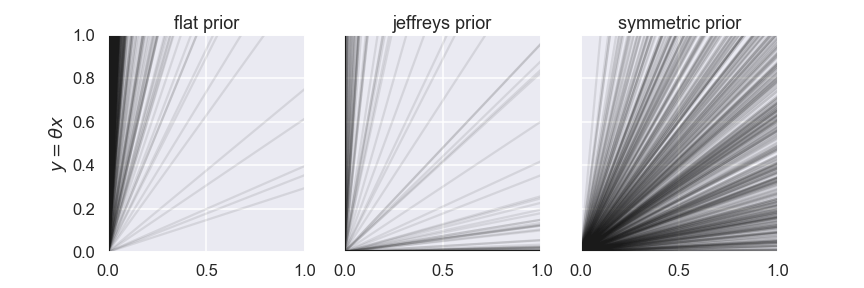
\includegraphics[width=0.8\linewidth]{fig/slope_priors.png}}
  \caption{
  100 samples of straight lines with fixed intercept equal to 0 and slopes sampled from three different pdfs. Note in particular the  prior preference for large slopes that results from using a uniform pdf.
  }
\end{figure}
%\clearpage % flush figures 



% !split
\section{The principle of maximum entropy}

Having dealt with ignorance, let us move on to more enlightened situations.

Consider a die with the usual six faces that was rolled a very large number of times. Suppose that we were only told that the average number of dots was 2.5. What (discrete) pdf would we assign? I.e. what are the probabilities $\{ p_i \}$ that the face on top had $i$ dots after a single throw?

% !split
The available information can be summarized as follows
\[
\sum_{i=1}^6 p_i = 1, \qquad \sum_{i=1}^6 i p_i = 2.5
\]
This is obviously not a normal die, with uniform probability $p_i=1/6$, since the average result would then be 3.5. But there are many candidate pdfs that would reproduce the given information. Which one should we prefer?

% !split
It turns out that there are several different arguments that all point in a direction that is very familiar to people with a physics background. Namely that we should prefer the probability distribution that maximizes an entropy measure, while fulfilling the given constraints. 

% !split
It will be shown below that the preferred pdf $\{ p_i \}$ is the one that maximizes

\[
Q\left( \{ p_i \} ; \lambda_0, \lambda_1 \right)
= -\sum_{i=1}^6 p_i \log(p_i) 
+ \lambda_0 \left( 1 - \sum_{i=1}^6 p_i \right)
+ \lambda_1 \left( 2.5 - \sum_{i=1}^6 i p_i \right),
\]
where the constraints are included via the method of \href{{https://en.wikipedia.org/wiki/Lagrange_multiplier}}{Lagrange multipliers}.

% !split
\subsection{The entropy of Scandinavians}

Let's consider another pdf assignment problem. This is originally the \emph{kangaroo problem} (Gull and Skilling, 1984), but translated here into a local context. The problem is stated as follows:

\begin{description}
\item[Information:] 
  70\% of all Scandinavians have blonde hair, and 10\% of all Scandinavians are left handed.

\item[Question:] 
  On the basis of this information alone, what proportion of Scandinavians are both blonde and left handed?
\end{description}

\noindent
% !split
We note that for any one given Scandinavian there are four distinct possibilities: 
\begin{enumerate}
\item Blonde and left handed (probability $p_1$).

\item Blonde and right handed (probability $p_2$).

\item Not blonde and left handed (probability $p_3$).

\item Not blonde and right handed (probability $p_4$).
\end{enumerate}

\noindent
% !split
The following 2x2 contingency table


\vspace{3mm}





\begin{tabular}{lcc}
\hline
\multicolumn{1}{c}{  } & \multicolumn{1}{c}{ Left handed } & \multicolumn{1}{c}{ Right handed } \\
\hline
Blonde     & $p_1$       & $p_2$        \\
Not blonde & $p_3$       & $p_4$        \\
\hline
\end{tabular}


\noindent


\vspace{3mm}


% !split
can be written in terms of a single variable $x$ due to the normalization condition $\sum_{i=1}^4 p_i = 1$, and the available information $p_1 + p_2 = 0.7$ and $p_1 + p_3 = 0.1$


\vspace{3mm}





\begin{tabular}{lcc}
\hline
\multicolumn{1}{c}{  } & \multicolumn{1}{c}{ Left handed } & \multicolumn{1}{c}{ Right handed } \\
\hline
Blonde     & $0 \le x \le 0.1$ & $0.7-x$      \\
Not blonde & $0.1-x$           & $0.2+x$      \\
\hline
\end{tabular}


\noindent


\vspace{3mm}


But which choice of $x$ is preferred?

% !split
\subsection{The monkey argument}

The monkey argument is a model for assigning probabilities to $M$ different alternatives that satisfy some constraint as described by $I$: 
\begin{itemize}
\item Monkeys throwing $N$ balls into $M$ equally sized boxes.

\item The normalization condition $N = \sum_{i=1}^M n_i$.

\item The fraction of balls in each box gives a possible assignment for the corresponding probability $p_i = n_i / N$.

\item The distribution of balls $\{ n_i \}$ divided by $N$ is therefore a candidate pdf $\{ p_i \}$.
\end{itemize}

\noindent
% !split
After one round the monkeys have distributed their (large number of) balls over the $M$ boxes.
\begin{itemize}
\item The resulting pdf might not be consistent with the constraints of $I$, however, in which case it should be rejected as a possible candidate.

\item After many such rounds, some distributions will be found to come up more often than others. The one that appears most frequently (and satisfies $I$) would be a sensible choice for $p(\{p_i\}|I)$.

\item Since our ideal monkeys have no agenda of their own to influence the distribution, this most favoured distribution can be regarded as the one that best represents our given state of knowledge.
\end{itemize}

\noindent
% !split
Now, let us see how this preferred solution corresponds to the pdf with the largest \texttt{entropy}. Remember in the following that $N$ (and $n_i$) are considered to be very large numbers ($N/M \gg 1$)

% !split
\begin{itemize}
\item There are $M^N$ different ways to distribute the balls.

\item The micro-states $\{ n_i\}$ are connected to the pdf $\{ p_i \}$ and the frequency of a given pdf is given by
\end{itemize}

\noindent
\[
F(\{p_i\}) = \frac{\text{number of ways of obtaining } \{n_i\}}{M^N}
\]
\begin{itemize}
\item The number of micro-states, $W(\{n_i\}))$, in the nominator is equal to $N! / \prod_{i=1}^M n_i!$. 

\item We express the logarithm of this number (where we use the Stirling approximation $\log(n!) \approx n\log(n) - n$ for large numbers, and there is a cancellation of two terms)
\end{itemize}

\noindent
\[
\log(W(\{n_i\})) = \log(N!) − \sum_{i=1}^M \log(n_i!) 
\approx N\log(N) - \sum_{i=1}^M n_i\log(n_i),
\]

% !split
\begin{itemize}
\item Therefore, the logarithm of the frequency of a given pdf is
\end{itemize}

\noindent
\[
\log(F(\{p_i\})) \approx -N \log(M) + N\log(N) - \sum_{i=1}^M n_i\log(n_i)
\]

Substituting $p_i = n_i/N$, and using the normalization condition finally gives
\[
\log(F(\{p_i\})) \approx -N \log(M) - N \sum_{i=1}^M p_i\log(p_i)
\]

% !split
We note that $N$ and $M$ are constants so that the preferred pdf is given by the $\{ p_i \}$ that maximizes
\[
S = - \sum_{i=1}^M p_i\log(p_i).
\]
You might recognise this quantity as the \emph{entropy} from statistical mechanics. The interpretation of entropy in statistical mechanics is the measure of uncertainty, which remains about a system after its observable macroscopic properties, such as temperature, pressure and volume, have been taken into account. For a given set of macroscopic variables, the entropy measures the degree to which the probability of the system is spread out over different possible microstates. Specifically, entropy is a logarithmic measure of the number of micro-states with significant probability of being occupied $S = -k_B \sum_i p_i \log(p_i)$, where $k_B$ is the Boltzmann constant.

% !split
\paragraph{Why maximize the entropy?}
\begin{itemize}
\item Information theory: maximum entropy=minimum information (Shannon, 1948).

\item Logical consistency (Shore {\&} Johnson, 1960).

\item Uncorrelated assignments related monotonically to $S$ (Skilling, 1988).
\end{itemize}

\noindent
Consider the third argument. Let us check it empirically to the problem of hair colour and handedness of Scandinavians. We are interested in determining $p_1 \equiv p(L,B|I) \equiv x$, the probability that a Scandinavian is both left-handed and blonde. However, in this simple example we can immediately realize that the assignment $p_1=0.07$ is the only one that implies no correlation between left-handedness and hair color. Any joint probability smaller than 0.07 implies that left-handed people are less likely to be blonde, and any larger vale indicates that left-handed people are more likely to be blonde.

% !split
So unless you have specific information about the existence of such a correlation, you should better not build it into the assignment of the probability $p_1$. 

\textbf{Question}: Can you show why $p_1 < 0.07$ and $p_1 > 0.07$ corresponds to left-handedness and blondeness being dependent variables?

% !split
Let us now empirically consider a few variational functions of $\{ p_i \}$ and see if any of them gives a maximum that corresponds to the uncorrelated assignment $x=0.07$, which implies $p_1 = 0.07, \, p_2 = 0.63, \, p_3 = 0.03, \, p_4 = 0.27$. A few variational functions and their prediction for $x$ are shown in the following table.


\vspace{3mm}





\begin{tabular}{ccc}
\hline
\multicolumn{1}{c}{ Variational function } & \multicolumn{1}{c}{ Optimal x } & \multicolumn{1}{c}{ Implied correlation } \\
\hline
$-\sum_i p_i \log(p_i)$     & 0.070     & None                \\
$\sum_i \log(p_i)$          & 0.053     & Negative            \\
$-\sum_i p_i^2 \log(p_i)$   & 0.100     & Positive            \\
$-\sum_i \sqrt{p_i(1-p_i)}$ & 0.066     & Negative            \\
\hline
\end{tabular}


\noindent


\vspace{3mm}


% !split
The assignment based on the entropy measure is the only one that respects this lack of correlations.


\begin{figure}[!ht]  % 
  \centerline{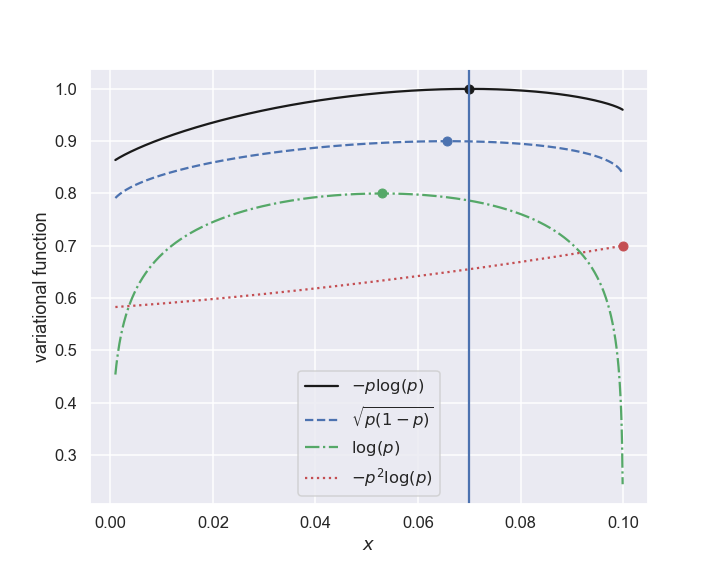
\includegraphics[width=0.8\linewidth]{fig/scandinavian_entropy.png}}
  \caption{
  Four different variational functions $f\left( \{ p_i \} \right)$. The optimal $x$ for each one is shown by a circle. The uncorrelated assignment $x=0.07$ is shown by a vertical line.
  }
\end{figure}
%\clearpage % flush figures 


% !split
\paragraph{Continuous case.}
Return to monkeys, but now with different probabilities for each bin.Then
\[
S= −\sum_{i=1}^M p_i \log \left( \frac{p_i}{m_i} \right),
\]
which is often known as the \emph{Shannon-Jaynes entropy}, or the \emph{Kullback number}, or the \emph{cross entropy} (with opposite sign).

Jaynes (1963) has pointed out that this generalization of the entropy, including a \emph{Leqesgue measure} $m_i$, is necessary when we consider the limit of continuous parameters. 
\[
S[p]= −\int p(x) \log \left( \frac{p(x)}{m(x)} \right).
\]

% !split
\begin{itemize}
\item In particular, $m(x)$ ensures that the entropy expression is invariant under a change of variables $x \to y=f(x)$.

\item Typically, the transformation-group (invariance) arguments are appropriate for assigning $m(x) = \mathrm{constant}$.

\item However, there are situations where other assignments for $m$ represent the most ignorance. For example, in counting experiments one might assign $m(N) = M^N / N!$ for the number of observed events $N$ and a very large number of intervals $M$.
\end{itemize}

\noindent
% !split
\subsection{Derivation of common pdfs using MaxEnt}

The principle of maximum entropy (MaxEnt) allows incorporation of further information, e.g.~constraints on the mean, variance, etc, into the assignment of probability distributions.

In summary, the MaxEnt approach aims to maximize the Shannon-Jaynes entropy and generates smooth functions.

% !split
\paragraph{Mean and the Exponential pdf.}
Suppose that we have a pdf $p(x|I)$ that is normalized over some interval $[ x_\mathrm{min}, x_\mathrm{max}]$. Assume that we have information about its mean value, i.e.,
\[
\langle x \rangle = \int x p(x|I) dx = \mu.
\]

Based only on this information, what functional form should we assign for the pdf that we will now denote $p(x|\mu)$? 

% !split
Let us use the principle of MaxEnt and maximize the entropy under the normalization and mean constraints. We will use Lagrange multipliers, and we will perform the optimization as a limiting case of a discrete problem; explicitly, we will maximize
\[
Q = -\sum_i p_i \log \left( \frac{p_i}{m_i} \right) + \lambda_0 \left( 1 - \sum_i p_i \right) + \lambda_1 \left( \mu - \sum_i x_i p_i \right).
\]

% !split
Setting $\partial Q / \partial p_j = 0$ we obtain
\[
p_j = m_j \exp \left[ -(1+\lambda_0) \right] \exp \left[ -\lambda_1 x_j \right].
\]

With a uniform measure $m_j = \mathrm{constant}$ we find (in the continuous limit) that
\[
p(x|\mu) = \mathcal{N} \exp \left[ -\lambda_1 x \right].
\]

% !split
The normalization constant (related to $\lambda_0$) and the remaining Lagrange multiplier, $\lambda_1$, can easily determined by fulfilling the two constraints. 

Assuming, e.g., that the normalization interval is $x \in [0, \infty[$ we obtain
\[
\int_0^\infty p(x|\mu) dx = 1 = \left[ -\frac{\mathcal{N}}{\lambda_1} e^{-\lambda_1 x} \right]_0^\infty = \frac{\mathcal{N}}{\lambda_1} \quad \Rightarrow \quad \mathcal{N} = \lambda_1.
\]
The constraint for the mean then gives
\[
\mu = \lambda_1 \int_0^\infty x  e^{-\lambda_1 x} dx = \lambda_1 \frac{1!}{\lambda_1^2}
= \frac{1}{\lambda_1}
\quad \Rightarrow \quad \lambda_1 = \frac{1}{\mu}.
\]

So that the properly normalized pdf from MaxEnt principles becomes the exponential distribution
\[
p(x|\mu) = \frac{1}{\mu} \exp \left[ -\frac{x}{\mu} \right].
\]

% !split
\paragraph{Variance and the Gaussian pdf.}
Suppose that we have information not only on the mean $\mu$ but also on the variance
\[
\left\langle (x-\mu)^2 \right\rangle = \int (x-\mu)^2 p(x|I) dx = \sigma^2.
\]

The principle of MaxEnt will then result in the continuum assignment
\[
p(x|\mu,\sigma) \propto \exp \left[ - \lambda_1 ( x - \mu )^2 \right].
\]

% !split
Assuming that the limits of integration are $\pm \infty$ this results in the standard Gaussian pdf
\[
p(x|\mu,\sigma) = \frac{1}{\sigma \sqrt{2\pi}} \exp \left[ - \frac{( x - \mu )^2}{2\sigma^2} \right].
\]

This indicates that the normal distribution is the most honest representation of our state of knowledge when we only have information about the mean and the variance.

% !split

\begin{notice_mdfboxadmon}[Notice]
These arguments extend easily to the case of several parameters. For example, considering $\{x_k\}$ as the data $\{ D_k\}$ with error bars $\{\sigma_k\}$ and $\{\mu_k\}$ as the model predictions, this allows us to identify the least-squares likelihood as the pdf which best represents our state of knowledge given only the value of the expected squared-deviation between our predictions and the data
\[
p\left( \{x_k\} | \{\mu_k, \sigma_k\} \right) = \prod_{k=1}^N \frac{1}{\sigma_k \sqrt{2\pi}} \exp \left[ - \frac{( x_k - \mu_k )^2}{2\sigma_k^2} \right].
\]

If we had convincing information about the covariance $\left\langle \left( x_i - \mu_i \right) \left( x_j - \mu_j \right) \right\rangle$, where $i \neq j$, then MaxEnt would assign a correlated, multivariate Gaussian pdf for $p\left( \{ x_k \} | I \right)$.
\end{notice_mdfboxadmon} % title: Notice



% !split
\paragraph{Counting statistics and the Poisson distribution.}
The derivation, and underlying arguments, for the binomial distribution and the Poisson statistic based on MaxEnt is found in Sivia, Secs 5.3.3 and 5.3.4.

% ------------------- end of main content ---------------

% #ifdef PREAMBLE
\end{document}
% #endif

